% Options for packages loaded elsewhere
\PassOptionsToPackage{unicode}{hyperref}
\PassOptionsToPackage{hyphens}{url}
%
\documentclass[
]{article}
\usepackage{amsmath,amssymb}
\usepackage{iftex}
\ifPDFTeX
  \usepackage[T1]{fontenc}
  \usepackage[utf8]{inputenc}
  \usepackage{textcomp} % provide euro and other symbols
\else % if luatex or xetex
  \usepackage{unicode-math} % this also loads fontspec
  \defaultfontfeatures{Scale=MatchLowercase}
  \defaultfontfeatures[\rmfamily]{Ligatures=TeX,Scale=1}
\fi
\usepackage{lmodern}
\ifPDFTeX\else
  % xetex/luatex font selection
\fi
% Use upquote if available, for straight quotes in verbatim environments
\IfFileExists{upquote.sty}{\usepackage{upquote}}{}
\IfFileExists{microtype.sty}{% use microtype if available
  \usepackage[]{microtype}
  \UseMicrotypeSet[protrusion]{basicmath} % disable protrusion for tt fonts
}{}
\makeatletter
\@ifundefined{KOMAClassName}{% if non-KOMA class
  \IfFileExists{parskip.sty}{%
    \usepackage{parskip}
  }{% else
    \setlength{\parindent}{0pt}
    \setlength{\parskip}{6pt plus 2pt minus 1pt}}
}{% if KOMA class
  \KOMAoptions{parskip=half}}
\makeatother
\usepackage{xcolor}
\usepackage[margin=1in]{geometry}
\usepackage{color}
\usepackage{fancyvrb}
\newcommand{\VerbBar}{|}
\newcommand{\VERB}{\Verb[commandchars=\\\{\}]}
\DefineVerbatimEnvironment{Highlighting}{Verbatim}{commandchars=\\\{\}}
% Add ',fontsize=\small' for more characters per line
\usepackage{framed}
\definecolor{shadecolor}{RGB}{248,248,248}
\newenvironment{Shaded}{\begin{snugshade}}{\end{snugshade}}
\newcommand{\AlertTok}[1]{\textcolor[rgb]{0.94,0.16,0.16}{#1}}
\newcommand{\AnnotationTok}[1]{\textcolor[rgb]{0.56,0.35,0.01}{\textbf{\textit{#1}}}}
\newcommand{\AttributeTok}[1]{\textcolor[rgb]{0.13,0.29,0.53}{#1}}
\newcommand{\BaseNTok}[1]{\textcolor[rgb]{0.00,0.00,0.81}{#1}}
\newcommand{\BuiltInTok}[1]{#1}
\newcommand{\CharTok}[1]{\textcolor[rgb]{0.31,0.60,0.02}{#1}}
\newcommand{\CommentTok}[1]{\textcolor[rgb]{0.56,0.35,0.01}{\textit{#1}}}
\newcommand{\CommentVarTok}[1]{\textcolor[rgb]{0.56,0.35,0.01}{\textbf{\textit{#1}}}}
\newcommand{\ConstantTok}[1]{\textcolor[rgb]{0.56,0.35,0.01}{#1}}
\newcommand{\ControlFlowTok}[1]{\textcolor[rgb]{0.13,0.29,0.53}{\textbf{#1}}}
\newcommand{\DataTypeTok}[1]{\textcolor[rgb]{0.13,0.29,0.53}{#1}}
\newcommand{\DecValTok}[1]{\textcolor[rgb]{0.00,0.00,0.81}{#1}}
\newcommand{\DocumentationTok}[1]{\textcolor[rgb]{0.56,0.35,0.01}{\textbf{\textit{#1}}}}
\newcommand{\ErrorTok}[1]{\textcolor[rgb]{0.64,0.00,0.00}{\textbf{#1}}}
\newcommand{\ExtensionTok}[1]{#1}
\newcommand{\FloatTok}[1]{\textcolor[rgb]{0.00,0.00,0.81}{#1}}
\newcommand{\FunctionTok}[1]{\textcolor[rgb]{0.13,0.29,0.53}{\textbf{#1}}}
\newcommand{\ImportTok}[1]{#1}
\newcommand{\InformationTok}[1]{\textcolor[rgb]{0.56,0.35,0.01}{\textbf{\textit{#1}}}}
\newcommand{\KeywordTok}[1]{\textcolor[rgb]{0.13,0.29,0.53}{\textbf{#1}}}
\newcommand{\NormalTok}[1]{#1}
\newcommand{\OperatorTok}[1]{\textcolor[rgb]{0.81,0.36,0.00}{\textbf{#1}}}
\newcommand{\OtherTok}[1]{\textcolor[rgb]{0.56,0.35,0.01}{#1}}
\newcommand{\PreprocessorTok}[1]{\textcolor[rgb]{0.56,0.35,0.01}{\textit{#1}}}
\newcommand{\RegionMarkerTok}[1]{#1}
\newcommand{\SpecialCharTok}[1]{\textcolor[rgb]{0.81,0.36,0.00}{\textbf{#1}}}
\newcommand{\SpecialStringTok}[1]{\textcolor[rgb]{0.31,0.60,0.02}{#1}}
\newcommand{\StringTok}[1]{\textcolor[rgb]{0.31,0.60,0.02}{#1}}
\newcommand{\VariableTok}[1]{\textcolor[rgb]{0.00,0.00,0.00}{#1}}
\newcommand{\VerbatimStringTok}[1]{\textcolor[rgb]{0.31,0.60,0.02}{#1}}
\newcommand{\WarningTok}[1]{\textcolor[rgb]{0.56,0.35,0.01}{\textbf{\textit{#1}}}}
\usepackage{graphicx}
\makeatletter
\def\maxwidth{\ifdim\Gin@nat@width>\linewidth\linewidth\else\Gin@nat@width\fi}
\def\maxheight{\ifdim\Gin@nat@height>\textheight\textheight\else\Gin@nat@height\fi}
\makeatother
% Scale images if necessary, so that they will not overflow the page
% margins by default, and it is still possible to overwrite the defaults
% using explicit options in \includegraphics[width, height, ...]{}
\setkeys{Gin}{width=\maxwidth,height=\maxheight,keepaspectratio}
% Set default figure placement to htbp
\makeatletter
\def\fps@figure{htbp}
\makeatother
\setlength{\emergencystretch}{3em} % prevent overfull lines
\providecommand{\tightlist}{%
  \setlength{\itemsep}{0pt}\setlength{\parskip}{0pt}}
\setcounter{secnumdepth}{-\maxdimen} % remove section numbering
\ifLuaTeX
  \usepackage{selnolig}  % disable illegal ligatures
\fi
\usepackage{bookmark}
\IfFileExists{xurl.sty}{\usepackage{xurl}}{} % add URL line breaks if available
\urlstyle{same}
\hypersetup{
  pdftitle={CodingChallenge4},
  pdfauthor={Muhtarin Khayer Brohee},
  hidelinks,
  pdfcreator={LaTeX via pandoc}}

\title{CodingChallenge4}
\author{Muhtarin Khayer Brohee}
\date{2025-02-27}

\begin{document}
\maketitle

{
\setcounter{tocdepth}{3}
\tableofcontents
}
\subsection{\texorpdfstring{\textbf{YAML
header}}{YAML header}}\label{yaml-header}

The YAML (Yet Another Markup Language) header is a metadata block at the
beginning of an R Markdown (.Rmd) document. It defines settings for the
document, such as the title, author, output format, and table of
contents. It is enclosed in triple dashes (---).

\subsection{\texorpdfstring{\textbf{Literate
programming}}{Literate programming}}\label{literate-programming}

Literate programming is an approach where code and natural language
explanations are combined in a single document. The goal is to create a
human-readable and reproducible document that integrates analysis with
documentation.

How does R Markdown support literate programming? - Code chunks
(`\texttt{\{r\}}) allow embedding of executable R code. - Markdown text
enables writing explanations, interpretation, and formatting. - Knit
output produces reports in HTML, PDF, or Word, making them easy to
share.

\href{https://pubmed.ncbi.nlm.nih.gov/34587775/}{Article Link}

\begin{Shaded}
\begin{Highlighting}[]
\NormalTok{DON\_data }\OtherTok{\textless{}{-}} \FunctionTok{read.csv}\NormalTok{(}\StringTok{"MycotoxinData.csv"}\NormalTok{, }\AttributeTok{na.strings =} \StringTok{"na"}\NormalTok{)}
\FunctionTok{str}\NormalTok{(DON\_data)}
\end{Highlighting}
\end{Shaded}

\begin{verbatim}
## 'data.frame':    375 obs. of  6 variables:
##  $ Treatment     : chr  "Fg" "Fg" "Fg" "Fg" ...
##  $ Cultivar      : chr  "Wheaton" "Wheaton" "Wheaton" "Wheaton" ...
##  $ BioRep        : int  2 2 2 2 2 2 2 2 2 3 ...
##  $ MassperSeed_mg: num  10.29 12.8 2.85 6.5 10.18 ...
##  $ DON           : num  107.3 32.6 416 211.9 124 ...
##  $ X15ADON       : num  3 0.85 3.5 3.1 4.8 3.3 6.9 2.9 2.1 0.71 ...
\end{verbatim}

\begin{Shaded}
\begin{Highlighting}[]
\CommentTok{\# Print column names to check for typos or formatting issues}
\FunctionTok{print}\NormalTok{(}\FunctionTok{colnames}\NormalTok{(DON\_data))}
\end{Highlighting}
\end{Shaded}

\begin{verbatim}
## [1] "Treatment"      "Cultivar"       "BioRep"         "MassperSeed_mg"
## [5] "DON"            "X15ADON"
\end{verbatim}

\begin{Shaded}
\begin{Highlighting}[]
\CommentTok{\# Show the first few rows of the dataset}
\FunctionTok{head}\NormalTok{(DON\_data)}
\end{Highlighting}
\end{Shaded}

\begin{verbatim}
##   Treatment Cultivar BioRep MassperSeed_mg   DON X15ADON
## 1        Fg  Wheaton      2      10.291304 107.3    3.00
## 2        Fg  Wheaton      2      12.803226  32.6    0.85
## 3        Fg  Wheaton      2       2.846667 416.0    3.50
## 4        Fg  Wheaton      2       6.500000 211.9    3.10
## 5        Fg  Wheaton      2      10.179167 124.0    4.80
## 6        Fg  Wheaton      2      12.044444  73.1    3.30
\end{verbatim}

\begin{Shaded}
\begin{Highlighting}[]
\CommentTok{\# Check the structure of the data}
\FunctionTok{str}\NormalTok{(DON\_data)}
\end{Highlighting}
\end{Shaded}

\begin{verbatim}
## 'data.frame':    375 obs. of  6 variables:
##  $ Treatment     : chr  "Fg" "Fg" "Fg" "Fg" ...
##  $ Cultivar      : chr  "Wheaton" "Wheaton" "Wheaton" "Wheaton" ...
##  $ BioRep        : int  2 2 2 2 2 2 2 2 2 3 ...
##  $ MassperSeed_mg: num  10.29 12.8 2.85 6.5 10.18 ...
##  $ DON           : num  107.3 32.6 416 211.9 124 ...
##  $ X15ADON       : num  3 0.85 3.5 3.1 4.8 3.3 6.9 2.9 2.1 0.71 ...
\end{verbatim}

\subsection{\texorpdfstring{\textbf{Plot}}{Plot}}\label{plot}

\begin{Shaded}
\begin{Highlighting}[]
\NormalTok{cbbPalette }\OtherTok{\textless{}{-}} \FunctionTok{c}\NormalTok{(}\StringTok{"\#000000"}\NormalTok{, }\StringTok{"\#E69F00"}\NormalTok{, }\StringTok{"\#56B4E9"}\NormalTok{, }\StringTok{"\#009E73"}\NormalTok{, }\StringTok{"\#F0E442"}\NormalTok{, }\StringTok{"\#0072B2"}\NormalTok{, }\StringTok{"\#D55E00"}\NormalTok{, }\StringTok{"\#CC79A7"}\NormalTok{)}


\NormalTok{DON\_plot }\OtherTok{\textless{}{-}} \FunctionTok{ggplot}\NormalTok{(DON\_data, }\FunctionTok{aes}\NormalTok{(}\AttributeTok{x =}\NormalTok{ Treatment, }\AttributeTok{y =}\NormalTok{ DON, }\AttributeTok{fill =}\NormalTok{ Cultivar)) }\SpecialCharTok{+}
  \FunctionTok{geom\_boxplot}\NormalTok{(}\AttributeTok{outliers =}\NormalTok{ T, }\AttributeTok{outlier.shape =} \DecValTok{15}\NormalTok{) }\SpecialCharTok{+}
  \FunctionTok{ylab}\NormalTok{(}\StringTok{"DON (ppm)"}\NormalTok{) }\SpecialCharTok{+}
  \FunctionTok{xlab}\NormalTok{(}\StringTok{""}\NormalTok{) }\SpecialCharTok{+}
  \FunctionTok{geom\_jitter}\NormalTok{(}\AttributeTok{pch =} \DecValTok{21}\NormalTok{, }\AttributeTok{position =} \FunctionTok{position\_jitterdodge}\NormalTok{(), }\AttributeTok{color =} \StringTok{"black"}\NormalTok{, }\AttributeTok{alpha =} \FloatTok{0.6}\NormalTok{) }\SpecialCharTok{+} 
  \FunctionTok{scale\_fill\_manual}\NormalTok{(}\AttributeTok{values =} \FunctionTok{c}\NormalTok{(cbbPalette[[}\DecValTok{3}\NormalTok{]], cbbPalette[[}\DecValTok{4}\NormalTok{]])) }\SpecialCharTok{+}
  \FunctionTok{theme\_classic}\NormalTok{() }\SpecialCharTok{+}
  \FunctionTok{facet\_wrap}\NormalTok{(}\SpecialCharTok{\textasciitilde{}}\NormalTok{Cultivar)}
\NormalTok{DON\_plot}
\end{Highlighting}
\end{Shaded}

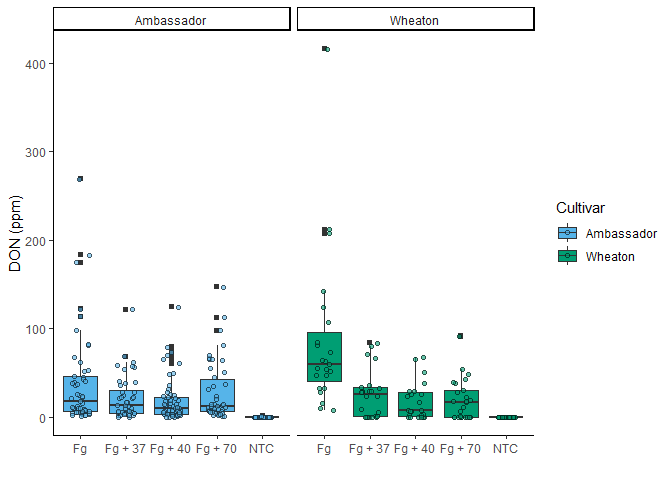
\includegraphics{Challagne4_files/figure-latex/data_plot-1.pdf}

\begin{Shaded}
\begin{Highlighting}[]
\NormalTok{DON\_data}\SpecialCharTok{$}\NormalTok{Treatment }\OtherTok{\textless{}{-}} \FunctionTok{factor}\NormalTok{(DON\_data}\SpecialCharTok{$}\NormalTok{Treatment, }\AttributeTok{levels =} \FunctionTok{c}\NormalTok{(}\StringTok{"NTC"}\NormalTok{, }\StringTok{"Fg"}\NormalTok{, }\StringTok{"Fg + 37"}\NormalTok{, }\StringTok{"Fg + 40"}\NormalTok{, }\StringTok{"Fg + 70"}\NormalTok{))}

\NormalTok{DON\_15 }\OtherTok{\textless{}{-}} \FunctionTok{ggplot}\NormalTok{(DON\_data, }\FunctionTok{aes}\NormalTok{(}\AttributeTok{x =}\NormalTok{ Treatment, }\AttributeTok{y =}\NormalTok{ X15ADON, }\AttributeTok{fill =}\NormalTok{ Cultivar)) }\SpecialCharTok{+}
  \FunctionTok{geom\_boxplot}\NormalTok{(}\AttributeTok{outliers =}\NormalTok{ F) }\SpecialCharTok{+}
  \FunctionTok{ylab}\NormalTok{(}\StringTok{"DON (ppm)"}\NormalTok{) }\SpecialCharTok{+}
  \FunctionTok{xlab}\NormalTok{(}\StringTok{""}\NormalTok{) }\SpecialCharTok{+}
  \FunctionTok{geom\_jitter}\NormalTok{(}\AttributeTok{pch =} \DecValTok{21}\NormalTok{, }\AttributeTok{position =} \FunctionTok{position\_jitterdodge}\NormalTok{(), }\AttributeTok{color =} \StringTok{"black"}\NormalTok{) }\SpecialCharTok{+} 
  \FunctionTok{scale\_fill\_manual}\NormalTok{(}\AttributeTok{values =} \FunctionTok{c}\NormalTok{(cbbPalette[[}\DecValTok{3}\NormalTok{]], cbbPalette[[}\DecValTok{4}\NormalTok{]])) }\SpecialCharTok{+}
  \FunctionTok{theme\_classic}\NormalTok{() }\SpecialCharTok{+}
  \FunctionTok{facet\_wrap}\NormalTok{(}\SpecialCharTok{\textasciitilde{}}\NormalTok{Cultivar)}
\NormalTok{DON\_15}
\end{Highlighting}
\end{Shaded}

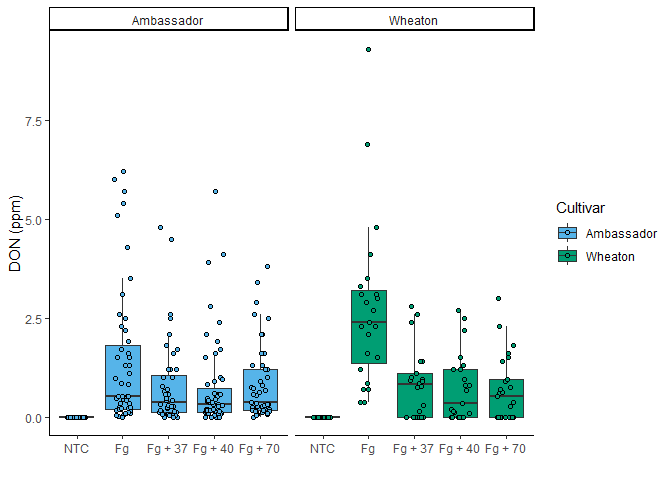
\includegraphics{Challagne4_files/figure-latex/data_plot-2.pdf}

\begin{Shaded}
\begin{Highlighting}[]
\NormalTok{seedmass }\OtherTok{\textless{}{-}} \FunctionTok{ggplot}\NormalTok{(DON\_data, }\FunctionTok{aes}\NormalTok{(}\AttributeTok{x =}\NormalTok{ Treatment, }\AttributeTok{y =}\NormalTok{ MassperSeed\_mg, }\AttributeTok{fill =}\NormalTok{ Cultivar)) }\SpecialCharTok{+}
  \FunctionTok{geom\_boxplot}\NormalTok{(}\AttributeTok{outliers =}\NormalTok{ F) }\SpecialCharTok{+}
  \FunctionTok{ylab}\NormalTok{(}\StringTok{"DON (ppm)"}\NormalTok{) }\SpecialCharTok{+}
  \FunctionTok{xlab}\NormalTok{(}\StringTok{""}\NormalTok{) }\SpecialCharTok{+}
  \FunctionTok{geom\_jitter}\NormalTok{(}\AttributeTok{pch =} \DecValTok{21}\NormalTok{, }\AttributeTok{position =} \FunctionTok{position\_jitterdodge}\NormalTok{(), }\AttributeTok{color =} \StringTok{"black"}\NormalTok{) }\SpecialCharTok{+} 
  \FunctionTok{scale\_fill\_manual}\NormalTok{(}\AttributeTok{values =} \FunctionTok{c}\NormalTok{(cbbPalette[[}\DecValTok{3}\NormalTok{]], cbbPalette[[}\DecValTok{4}\NormalTok{]])) }\SpecialCharTok{+}
  \FunctionTok{theme\_classic}\NormalTok{() }\SpecialCharTok{+}
  \FunctionTok{facet\_wrap}\NormalTok{(}\SpecialCharTok{\textasciitilde{}}\NormalTok{Cultivar)}
\NormalTok{seedmass}
\end{Highlighting}
\end{Shaded}

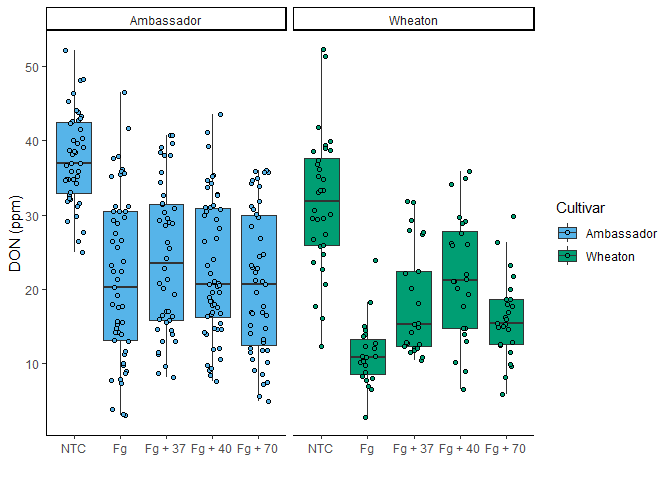
\includegraphics{Challagne4_files/figure-latex/data_plot-3.pdf}

\subsubsection{\texorpdfstring{\textbf{Combined
plot}}{Combined plot}}\label{combined-plot}

\begin{Shaded}
\begin{Highlighting}[]
\FunctionTok{ggarrange}\NormalTok{(DON\_plot, DON\_15, seedmass, }\AttributeTok{labels =} \StringTok{"auto"}\NormalTok{, }\AttributeTok{ncol =} \DecValTok{3}\NormalTok{, }\AttributeTok{nrow =} \DecValTok{1}\NormalTok{, }\AttributeTok{common.legend =}\NormalTok{ T)}
\end{Highlighting}
\end{Shaded}

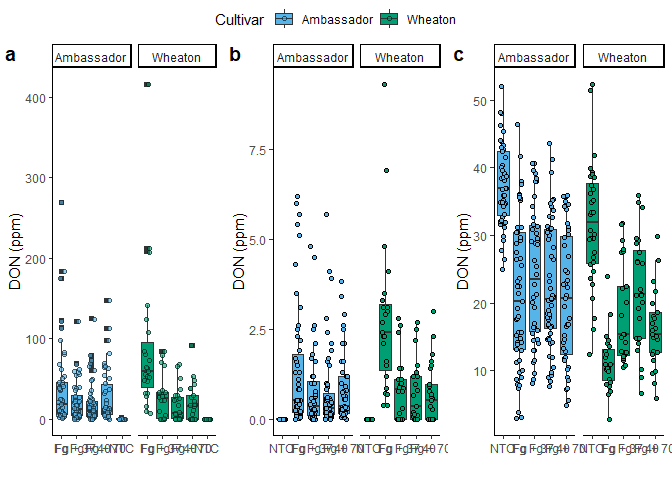
\includegraphics{Challagne4_files/figure-latex/combined_plot-1.pdf}

\subsection{\texorpdfstring{\textbf{Statistical
comparison}}{Statistical comparison}}\label{statistical-comparison}

\begin{Shaded}
\begin{Highlighting}[]
\NormalTok{stats\_donplot }\OtherTok{\textless{}{-}}\NormalTok{ DON\_plot }\SpecialCharTok{+} 
  \FunctionTok{geom\_pwc}\NormalTok{(}\FunctionTok{aes}\NormalTok{(}\AttributeTok{group =}\NormalTok{ Treatment), }\AttributeTok{method =} \StringTok{"t\_test"}\NormalTok{, }\AttributeTok{label =} \StringTok{"\{p.adj.format\}\{p.adj.signif\}"}\NormalTok{, }\AttributeTok{p.adjust.method =} \StringTok{"fdr"}\NormalTok{)}

\NormalTok{stats\_DON\_15 }\OtherTok{\textless{}{-}}\NormalTok{ DON\_15 }\SpecialCharTok{+} 
  \FunctionTok{geom\_pwc}\NormalTok{(}\FunctionTok{aes}\NormalTok{(}\AttributeTok{group =}\NormalTok{ Treatment), }\AttributeTok{method =} \StringTok{"t\_test"}\NormalTok{, }\AttributeTok{label =} \StringTok{"\{p.adj.format\}\{p.adj.signif\}"}\NormalTok{, }\AttributeTok{p.adjust.method =} \StringTok{"fdr"}\NormalTok{)}

\NormalTok{stats\_seedmass }\OtherTok{\textless{}{-}}\NormalTok{ seedmass }\SpecialCharTok{+} 
  \FunctionTok{geom\_pwc}\NormalTok{(}\FunctionTok{aes}\NormalTok{(}\AttributeTok{group =}\NormalTok{ Treatment), }\AttributeTok{method =} \StringTok{"t\_test"}\NormalTok{, }\AttributeTok{label =} \StringTok{"\{p.adj.format\}\{p.adj.signif\}"}\NormalTok{, }\AttributeTok{p.adjust.method =} \StringTok{"fdr"}\NormalTok{)}
\end{Highlighting}
\end{Shaded}


\end{document}
